Let $ P_1,P_2,\ldots,P_8$ be $ 8$ distinct points on a circle. Determine the number of possible configurations made by drawing a set of line segments connecting pairs of these $ 8$ points, such that: $ (1)$ each $ P_i$ is the endpoint of at most one segment and $ (2)$ no two segments intersect. (The configuration with no edges drawn is allowed. An example of a valid configuration is shown below.)


\begin{center}
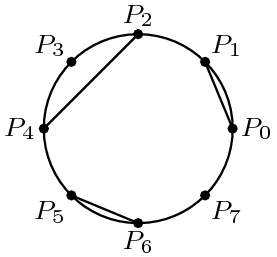
\includegraphics[width = 27.6mm]{img/fig0.png}
\end{center}